\documentclass[12pt, twoside]{report}

\usepackage{color}
\usepackage{fancyhdr}
\usepackage{float}
\usepackage[a4paper, width=150mm, top=25mm, bottom=25mm]{geometry}
\usepackage[nopostdot]{glossaries}
\usepackage{graphicx}
\usepackage[hyphens]{url}
\usepackage{hyperref}
\usepackage[utf8]{inputenc}
\usepackage{listings}
\usepackage{lmodern}
\usepackage{titlesec}

\pagestyle{fancy}

\newcommand{\projecttitle}{Distributed Programs}
\newcommand{\projectsubtitle}
    {Compiling a CSP-like language for a distributed system}

%\titleformat{\chapter}
%    {\Large\bfseries}    % Format
%    {\huge\thechapter)}  % Label
%    {20pt}               % Separation
%    {\huge}              % Before-code
%\titleclass{\chapter}{straight}
\titlespacing*{\chapter}{0pt}{30pt}{10pt}

% Code listing style.
\definecolor{label}{rgb}{0.0, 0.5, 0.8}
\definecolor{comment}{rgb}{0.0, 0.5, 0.0}
\definecolor{keyword}{rgb}{0.0, 0.0, 0.5}
\definecolor{string}{rgb}{0.4, 0.4, 0.4}
\definecolor{numbers}{rgb}{0.7, 0.7, 0.7}
\lstset{
  basicstyle=\fontsize{8pt}{1em}\ttfamily,
  commentstyle=\color{comment},
  keywordstyle=\bfseries\color{keyword},
  numbers=left,
  numberstyle=\color{numbers},
  stringstyle=\color{string},
  xleftmargin=0.75cm
}

\lstdefinelanguage{occam}{
  keywords={
    AFTER, ALT,   AND,    ANY,  AT,    BYTE, CHAN,
    CONST, DEF,   FALSE,  FOR,  IF,    NOT,  OR,
    PAR,   PLACE, PLACED, PRI,  PROC,  SEQ,  SKIP,
    STOP,  TABLE, TIME,   TRUE, VALUE, VAR,  WHILE
  },
  morecomment=[l]{--},
  morestring=[b]',
  morestring=[b]",
  sensitive=true
}

\lstdefinelanguage{assembly}{
  keywords={
    % Direct operations.
    j, ldlp, pfix, ldnl, ldc, ldnlp, nfix, ldl, adc, call, cj, ajw, eqc, stl,
    stnl, opr,
    % Indirect operations.
    add, and, diff, diss, div, dup, enbs, endp, gt, lb, ldpi, lend, mint, mul,
    not, or, outword, rem, ret, rev, runp, sb, shl, shr, startp, stopp, sub,
    wsub, xor,
    % Debugging operations.
    putc, puts, printdec, printhex, printr
  },
  identifierstyle=\color{label},
  morecomment=[l]{\#},
  sensitive=true
}

\lstdefinelanguage{json}{
  morestring=[b]"
}

\lstdefinelanguage{enum}{
  morecomment=[l]{\#}
}

\makeglossaries

\newglossaryentry{fsa}{
  name = Finite State Automata,
  text = finite state automata,
  description = {
    Given an alphabet $\Sigma$, a finite state automaton can be defined by a
    collection of states $S$, a starting state $s_0 \in S$, a set of accepting
    states $A \subseteq S$, and a transfer function
    $\delta ~:~ S \times S \to S$.
  }
}

\newglossaryentry{regex}{
  name = Regular Expression,
  text = regular expression,
  description = {
    A textual representation of \gls{reglang}. Common dialects of regular
    expressions include: character classes such as \texttt{[a-z0-9]}, which
    would match any lowercase alphabetic character or digit; $e_1$ \texttt{|}
    $e_2$ for the union of the languages expressed by $e_1$ and $e_2$; $e_1^*$
    for the language of \textit{zero} or more repetitions of $e_1$; and $e_1^+$
    for the language of \textit{one} or more repetitions of $e_1$.
  }
}

\newglossaryentry{reglang}{
  name = Regular Language,
  text = regular language,
  description = {
    The collection of regular languages is exactly the collection of languages
    which can be recognised by \textit{\gls{fsa}}. A regular language might be
    used to match simple patterns such as email addresses, which consist of a
    clear sequence of components that can only happen in a particular order.
    However, more complicated patterns such as matched nested brackets cannot be
    described or recognised by any regular language, as the corresponding
    automata would have to be infinite in size in order to deal with the
    arbitrarily deep nesting. Perhaps the most common way of expressing a
    regular language is to use \textit{\gls{regex}}.
  }
}

\newglossaryentry{cflang}{
  name = Context-Free Language,
  text = context-free language,
  description = {
    The collection of context-free languages is a strict superset of the
    collection of \gls{reglang}.
  }
}

\newglossaryentry{cfg}{
  name = Context-Free Grammar,
  text = context-free grammar,
  description = {
    Just as \gls{regex}s are a way of describing \gls{reglang}s, context-free
    grammars are a way of describing \gls{cflang}s. A context-free grammar is
    made up of a collection of rules describing reductions. The rule
    $A \to \texttt{abc}$ states that the grammar symbol $A$ can be reduced to
    the collection of language symbols \texttt{abc}. Rules may be recursive, and
    may reference other rules. For example, the rule
    $A \to \texttt{(}A\texttt{)}A ~\texttt{|}~ \epsilon$ states that $A$ may be
    reduced to either the expression $\texttt{(}A\texttt{)}A$, or to the empty
    string which is denoted by $\epsilon$. Context-free grammars are therefore
    able to match patterns such as nested brackets, making them far more
    suitable for programming languages than \gls{reglang}s.
  }
}

\newglossaryentry{lexing}{
  name = Lexing,
  text = lexing,
  description = {
    The process of converting a stream of characters into a (smaller) stream of
    tokens. In the context of compilers, these tokens are usually things such as
    keywords, identifiers, and numbers.
  }
}

\newglossaryentry{transputer}{
  name = Transputer,
  text = transputer,
  description = {
    A processor architecture developed in the 1980s which was designed alongside
    Occam with the intention of being programmed exclusively in Occam. See
    \ref{transputer} for a more detailed description.
  }
}

\newglossaryentry{direct}{
  name = Direct Instruction,
  text = direct instruction,
  description = {
    In the Transputer instruction set, Direct Instructions are those which can
    be executed without use of the \texttt{OPR} instruction. There are 13 such
    instructions, each with a 4-bit operand which can be extended via the
    \gls{prefix-instructions}.
  }
}

\newglossaryentry{prefix-instructions}{
  name = Prefix Instructions,
  text = prefix instructions,
  description = {
    In the Transputer instruction set, there are two prefix instructions:
    \texttt{PFIX} (Prefix) and \texttt{NFIX} (Negative Prefix). These
    instructions are used to extend the operand beyond 4-bits by allowing
    additional bits to be shifted into the operand register prior to executing
    the operation.
  }
}

\newglossaryentry{indirect}{
  name = Indirect Instruction,
  text = indirect instruction,
  description = {
    In the Transputer instruction set, Indirect Instructions are those which are
    executed via the \texttt{OPR} instruction. Exactly 16 of these require only
    a single byte (the operation number fits inside the 4-bit operand of the
    \texttt{OPR} instruction), but an arbitrarily large number of additional
    instructions can be used via the \gls{prefix-instructions}.
  }
}

\newglossaryentry{workspace}{
  name = Workspace,
  text = workspace,
  description = {
    A process running on the Transputer is associated with a workspace. The
    workspace is effectively a stack pointer, but this location in memory is
    also used to store additional information about halted processes. The
    address of the workspace pointer is required to be word-aligned. When
    the combined with the process priority level via bitwise-or, the result is
    referred to as the workspace descriptor.
  }
}

\newglossaryentry{ast}{
  name = Abstract Syntax Tree,
  text = abstract syntax tree,
  description = {
    The Abstract Syntax Tree (often abbreviated to AST) is the abstract
    representation of the source code. Each functional construct in the language
    is likely to have a corresponding node in the abstract syntax. The AST is
    generated by the parser, and serves as the input to semantic analysis or
    code generation.
  }
}

\newglossaryentry{risc}{
  name = Reduced Instruction Set Computer,
  text = RISC,
  description = {
    A Reduced Instruction Set Computer (RISC) is a computer for which the
    instruction set consists of very simple instructions. The main advantage of
    such an instruction set is that each instruction only utilises a small
    amount of the hardware at a time, allowing for the processor to be heavily
    pipelined to increase the performance.
  }
}

\newglossaryentry{mnemonic}{
  name = Mnemonic,
  text = mnemonic,
  description = {
    In the context of assemblers, a mnemonic is a name associated with the
    opcode for an instruction, which is intended to be easier for a human to
    remember.
  }
}

\newglossaryentry{vm}{
  name = Virtual Machine,
  text = virtual machine,
  description = {
    The Virtual Machine interprets and executes program bytecode. See \ref{vm}
    for details.
  }
}

\newglossaryentry{lazy-eval}{
  name = Lazy Evaluation,
  text = lazy evaluation,
  description = {
    Intuitively, lazy evaluation is a reduction strategy which only performs
    work that is essential for computing the overall result. This results in a
    slight performance overhead in cases where all intermediate calculations are
    necessary, but can often significantly reduce the computational complexity
    of na\"ive implementations.
  }
}

\glossarystyle{altlist}


\begin{document}
  \begin{titlepage}
  \newgeometry{margin=1in}
    \begin{center}
      \vspace*{1cm}

      \huge
      \textbf{\projecttitle}

      \vspace{0.5cm}
      \large \projectsubtitle

      \vspace{1.5cm}

      \textbf{Joe Fowler}

      Keble College

      \vfill

      \includegraphics[width=0.3\textwidth]{images/OxfordLogo}

      \vspace{1cm}

      \large
      Department of Computer Science\\
      University of Oxford\\
      United Kingdom\\
      2016-05-23
    \end{center}
  \restoregeometry
\end{titlepage}


  \newpage
  \thispagestyle{empty}
  \mbox{}
  \newpage

  \setcounter{page}{1}
  \thispagestyle{plain}

\begin{center}
  \Large
  \textbf{\projecttitle}

  \vspace{0.4cm}
  \large \projectsubtitle

  \vspace{0.4cm}
  \textbf{Joe Fowler}

  \vspace{0.9cm}
  \textbf{Abstract}
\end{center}
{}
...


  \tableofcontents
  \clearpage

  \chapter{Introduction} \label{introduction}
    


  \chapter{Background} \label{background}
    This project has a heavy focus on the programming language Occam, and the
Transputer microprocessor that the language was designed for. This section
explores the details relevant to the design of an Occam compiler, and of a
Transputer emulator.

\section{Formal Languages}

A key part of understanding any compiler is knowledge of some of the different
classes of formal language. The two that are most important to compilers are
\textit{\gls{reglang}s} and \textit{\gls{cflang}s}.

\subsection{Regular Languages}

Regular Languages come into compilers at the \textit{\gls{lexing}} stage, as most
languages can be tokenised in such a way that each token can be matched by a
\gls{reglang}. In this project, regular expressions are not explicitly used as
part of the implementation, but serve as a manner of summarising how the input
is split into tokens.

\subsection{Context-Free Languages}

A lot of programming languages are, at their heart, context-free. The advantage
of this is that the structure of \textit{\gls{cfg}s} makes them ideal for
compiling code: the individual rules can each be matched by code which compiles
that particular construct. The grammar rules for the language are defined as a
context-free grammar, and the compiler implements a top-down backtracking
technique in order to parse them.

\section{Occam}

Occam is a procedural concurrent programming language that was introduced in the
1980s. The language has a very recognisable syntax in which indentation is used
to denote blocks of related code, and communication between concurrent threads
is performed via message passing through CSP-like channels. For the purpose of
this project and for the sake of simplicity, I will be focusing on the first
version of Occam.

\subsection{Basic Syntax}

By today's standards, Occam has an unusual syntax:

\begin{lstlisting}[language=occam]
PROC foo(VALUE a, b, CHAN c, d) =
  PAR i = [0 FOR n]  -- Replicated parallel.
    SEQ              -- Explicit sequence.
      VAR x :        -- Declare variable x.
      bar(x, i)      -- Call procedure bar.
      IF             -- If statement.
        x < b        -- if (x < b) {
          c ! a      --   Output a to channel c.
        x >= b       -- } else if (x >= b) {
          d ! ANY    --   Output something (it doesn't matter what) to d.
:                    -- }

PROC bar(VAR x, VALUE i) =          -- Occam has no operator precedence:
  x := ((i * i) \ (i + i + i)) - i  -- It is necessary to bracket all except
:                                   -- sequences of some associative operator.

CHAN c, d :
VAR x, e, f :
PAR
  foo(-1, 1, c, d)   -- Run the process foo.
  SEQ i = [0 FOR n]  -- Loop n times:
    ALT              -- Alternative: perform one of the following:
      c ? x          -- Read a value x from c.
        e := e + x
      d ? ANY        -- Read something (it doesn't matter what) from d.
        f := f + 1
\end{lstlisting}

The above (meaningless) program demonstrates some of the details of the
language. Note that unlike many other languages, Occam requires sequences of
statements to be explicitly denoted by the keyword \texttt{SEQ}. In fact, the
textual syntax is remarkably similar to the abstract syntax that one might
expect to find in the compiler.

\section{The Transputer}

The Transputer was an advanced processor which presented several advanced
features aimed at facilitating concurrent programming. The processor supported
synchronous communication over each of its four external serial connections, as
well as time-sliced concurrent processes, all through microcoded instructions
that made it possible to do these things with only a handful of assembly.

More like a microprocessor than merely a CPU, the Transputer incorporated all
the circuitry required for it to function, and it was the intention of INMOS to
market the Transputer as a one-size-fits-all solution for both areas. The aim
was for each unit to cost no more than a few dollars, and for it to be used for
everything from basic device controllers to hosting operating systems.

\subsection{Instruction Set}

The Transputer had an unusually high clock speed for its time. This was mostly
possible due to it being a RISC architecture. The transputer supports 13
\textit{\gls{direct}s}, each 8 bits, in its instruction set. Each of these
has room for a 4-bit operand. If room for an operand larger than 4 bits is
required then one of the additional instructions \texttt{PFIX} (prefix) or
\texttt{NFIX} (negative prefix) can be used to prepend additional bits. In
addition to these instructions, there is also the \texttt{OPR} (operate)
instruction, which interprets its operand as one of the many
\textit{\gls{indirect}s} available, and executes it.

\subsection{Registers}

The transputer does not have random access registers like many modern RISC
architectures. Instead, it has a small collection of single-purpose registers
which are accessed via specific instructions, and three general-purpose
registers which are arranged in a stack. However, some instructions can clobber
the contents of this stack, so it is intended to be used only for passing
arguments to instructions. Instead, the programmer should store the results of
all computations into the \textit{\gls{workspace}} of the process. This is
similar to a conventional falling stack, but with the added detail that the
workspace uniquely identifies the process that it belongs to.

\subsection{Inter-process Communication}

As mentioned above, inter-process communication on the Transputer is achieved
via message passing. What makes this impressive is that to the programmer, there
is no difference (other than a memory address) between communicating between
processes on the same Transputer, and communicating between two different
Transputers. The instructions remain the same, and the difference is handled in
the microcode. If one process tries to send a message to another before the
second is ready for it, then the first will wait until the second is ready
before sending, and it will not proceed until the second has received the
message. In this way, the channels can be used to synchronise separate threads.

\subsection{Concurrency}

The Transputer provides a small selection of instructions which schedule new
processes to run alongside the current. Only one process is truly running at any
given time, but the processor time-slices between the scheduled processes so
that all may proceed. It does so when particular instructions are performed
which can cause the process to yield control to another. If a process performs a
blocking action (eg. waiting upon a channel) then it will be descheduled until
it can proceed. The Transputer has two different priority levels which processes
can be executed at: low-priority and high-priority. If there is any
high-priority process which is currently scheduled, then it is guaranteed to
make progress before any low-priority process.

The processes are arranged in two linked lists; one for each priority level.
When a process is scheduled, it appears in one of these linked lists. The front
and back pointers of each list are stored in registers. Each pointer consists of
the address of the workspace of some process, with the priority of the process
encoded in the least significant bit of the workspace address\footnote{Workspace
addresses must be aligned to word boundaries, so the least significant two bits
can be safely ignored when recovering the workspace address.}. The workspace of
a descheduled process contains additional information below the workspace
pointer, such as the \texttt{Iptr} (instruction pointer) of the descheduled
process.

\subsection{Parallelism}

Although it has built-in support for having multiple processes running at once,
the Transputer does not implement true parallelism. The multiprocessing is
achieved by rapid switching between the active processes, and so there is no
performance gain made by having two processes instead of one. Rather, the point
of the multiprocessing support is to help break down programs into more
manageable processes which can act concurrently.

However, this does not mean that the Transputer is incapable of true
parallelism: the microprocessor comes equipped with four external serial
connections over which the Transputer is able to perform synchronous channel
operations. From the perspective of the programmer, the manner by which this is
achieved is exactly the same as if the Transputer was performing communication
over an internal channel, which means that the code does not have to be compiled
with special knowledge of which channels are internal and which are external.

By combining several Transputers together, true parallelism is therefore quite
achievable.


  \chapter{Requirements} \label{requirements}
    The purpose of this project is to explore the intricacies of compiling an
Occam-like language. Given the highly concurrent nature of Occam, it seems
natural to consider the possibility of making the runtime environment
distributed. This chapter will formally set out the scope of the project, and
address which features will be implemented and with what priority.

\section{Occam Features}

The compiler implemented in this project aims to implement a large subset of
the functionality of Occam 1, as well as a handful of customisations. Common
language features are not the focus of this project. Instead, the features
implemented in the compiler are the ones which are most interesting. Most of the
time spent on the compiler was aimed at making it pleasant to use, and on making
the runtime environment featureful and efficient.

\subsection{Language Features}

These are features which could reasonably be considered as fundamental to Occam.
The main features which have been implemented are:
\begin{itemize}
  \item Integer variables.
  \item Channels.
  \item One-dimensional arrays (of integers or channels).
  \item \texttt{SEQ}, \texttt{PAR}, and \texttt{IF} constructs, both with and
        without replication.
  \item \texttt{WHILE} and \texttt{ALT} constructs.
\end{itemize}
In addition to these features, I have implemented an extension to the language,
the \texttt{DIST PAR} construct, which allows the programmer to distribute
a task across an arbitrarily large number of workers. The construct works in the
same way as a PAR construct, but distributes the sub-processes across multiple
machines rather than running them all locally. These processes may not read or
write to variables defined outside their own scope, but they may communicate via
channels that were defined outside their scope. The runtime needed to support
this functionality is described in more detail below.

\subsection{Features Beyond Scope} \label{beyond-scope}

The following Occam features are outside the scope of this project:
\begin{itemize}
  \item Time-related functionality such as timer input or delays.
  \item Procedures, which provide no new functionality to the language.
  \item Replicated \texttt{ALT} constructs.
\end{itemize}
These features are ones which are time-consuming or challenging to implement,
but are not necessary for the compiler to be useful.

\section{Runtime Environment}

The compiler transforms the program source into an executable format which can
be understood by the virtual machine. It is the task of the overall runtime
environment to allow multiple instances of the virtual machine to interact with
each other.

\subsection{Virtual Machine} \label{vm}

The \textit{\gls{vm}} should be capable of executing code which is intended to
run on a single processor. This does not mean that it is limited to a single
process, however, rather that it only provides concurrency rather than
parallelism. This is modelled on the instruction set of the \gls{transputer},
with appropriate modifications to support the language extensions described
above. Some instructions that are unused by the compiler have been omitted to
keep the VM simple.

\subsection{Distributed Runtime System} \label{dist-system}

Since Occam processes communicate via channels rather than by sharing memory, it
is relatively easy to imagine these channels connecting processes on separate
threads, or even separate machines, through use of traditional approaches such
as atomic memory operations, mutexes, or even network sockets. If some mechanism
for using these more advanced channels were built into the language, then a
programmer could write separate Occam programs for a collection of VM instances,
and have them collaborate. The programmer would have to consider the complexity
of each of the parallel tasks and organise the code such that each of the
instances had a fair share of the load.

However, sometimes it is not possible to predict details such as this. The load
may vary, or the number of machines available for running the program may
change. Factors such as user input or other real-world data could easily change
the load characteristics of the software when values stray from ranges that the
programmer predicted. These issues make it hard for a programmer to design
a system with enough flexibility to handle all different parameters.

This is where the language extensions come into play. By removing the
responsibility of process placement from the programmer, the runtime system is
able to make that decision based on the properties of each process, and on the
load of each server at that moment. Additionally, this means that a program can
be run on a different number of machines without changing the source code.

For this reason, the runtime system is capable of supporting communication
between a large number of instances which may span several machines. When new
processes are constructed via the \texttt{DIST PAR} construct, the runtime
system can make an informed decision about \textit{where} the process should be
started. In a production system, it would be desirable to also handle failure
cases such as loss of connection or hardware failure, but this is beyond the
scope of this project; all hardware is assumed to be perfectly reliable, and all
connections are assumed to be unbroken.


  \chapter{Design} \label{design}
    The implementation for this project will be broken into three main parts: the
Occam compiler, the \gls{transputer} virtual machine, and the runtime systems.
These components are all conceptually separated, so it is convenient to separate
them in the implementation to make them more understandable. The compiler for
the project is written in \texttt{Haskell}, whilst the virtual machine and the
runtime systems are both written in \texttt{C++}.

\section{Compiler}

The Occam syntax is designed such that the indentation very much determines the
structure of the program. Whilst this is convenient for humans, it presents an
inconvenience for the compiler: this syntax is \textit{not} context-free. The
meaning of indentation on one line depends upon the indentation on the
surrounding lines. If it has increased, then a new block as started; if it has
decreased, one has ended.

Luckily, it is possible to transform the source code at an early stage so that
it is then context-free. This makes it much more simple to parse. The
transformation is described in the first three sections below.

\subsection{Lexer}

The Lexer is responsible for performing the first stage of the parsing. The
plain text of the source code is taken as input, and a stream of tokens is
produced. Each token consists of one lexical unit from the source code. At this
stage each unit is a terminal token, meaning that there is no sub-structure in
a given token, but a clearly defined meaning.

The Occam syntax has only a handful of different token types:
\begin{itemize}
  \item \texttt{CHAR c} - A character literal, e.g. \texttt{'a'}.
  \item \texttt{COMMENT} - A comment, e.g. \texttt{-- foo}.
  \item \texttt{IDENT x} - An identifier, e.g. \texttt{bar}.
  \item \texttt{INTEGER i} - An integer literal, e.g. \texttt{123}.
  \item \texttt{KEYWORD k} - A program keyword, e.g. \texttt{SEQ}.
  \item \texttt{STRING s} - A string literal, e.g. \texttt{"Hello, World!"}.
  \item \texttt{SYMBOL s} - An operator symbol, e.g. \texttt{*} or \texttt{:=}.
\end{itemize}
In addition to these tokens, there are two more which are only important for
parsing the indentation of the program:
\begin{itemize}
  \item \texttt{NEWLINE} - A line break.
  \item \texttt{SPACES n} - A sequence of \texttt{n} spaces.
\end{itemize}
These tokens are removed or substituted in the Indentation Parsing stage.

\subsection{Indentation Parsing}

The indentation parser takes the token stream generated by the Lexer, and
produces a different token stream which can be parsed in a context-free manner.
Most tokens are passed through this stage unmodified; the only tokens which are
changed or removed are the \texttt{COMMENT}, \texttt{NEWLINE} and
\texttt{SPACES} tokens.

Indentation parsing is achieved as follows: the token stream is split into
groups of tokens, breaking at each \texttt{NEWLINE} token; the \texttt{COMMENT}
tokens are removed, and \texttt{SPACES} tokens in each line are removed, unless
they are indentation\footnote{i.e. they are the first token on a line, and the
next token is not whitespace.}; finally, the remaining \texttt{SPACES} tokens
are all indentation, and can be converted into \texttt{INDENT} and
\texttt{DEDENT} tokens whenever the level of indentation is increased or
decreased between lines. By performing this transformation, the task of parsing
the new token stream is now context-free.

\subsection{Syntax Parsing}

Taking the output of the indentation parser as input, it is now possible to
parse the grammar with a collection of \gls{cfg} rules. The full grammar for
Occam is quite long and complex, so the majority of these rules were sourced in
part from \cite[p.~124]{jones}, and otherwise from
\cite[p.~106]{occ21}\footnote{This manual is actually for a later version of
Occam, which means that although many of the grammar rules do apply to the first
version of Occam, it contains several that do not.}.

One possibility for parsing would be to use an existing utility such as
\textit{Happy}\footnote{\url{https://www.haskell.org/happy/}} to generate a
parser from the grammar. However, such utilities often require a great deal of
effort in order to have them correctly track line numbers and columns for the
sake of generating understandable syntax errors, so I have elected to implement
the parser from scratch.

The parser consists of two main parts. The first part is a collection of
functions which describe parsing behaviour for each of a collection of
context-free combinators, as well as reduction rules which are used to construct
the \textit{\gls{ast}} from the source. This loosely acts as an alternative to a
parser generator, but makes it much easier to track source locations for error
messages. The second part is an expression of each of the grammar rules of Occam
in terms of these combinators. Together, they form a complete parser for the
Occam language.

\subsection{Semantic Checking}

Successful completion of the parsing phase implies that the source code is
grammatically sound. However, it is still possible that the source code does not
make sense. Consider the following example:
\begin{lstlisting}[language=occam]
CHAN c :
SEQ
  c := 2
\end{lstlisting}
Grammatically, there is nothing wrong with the line \texttt{c := 2}. However,
semantically, it makes no sense to assign an integer value to a channel. Thus,
it is necessary to perform semantic analysis to ensure that the program makes
sense. The list of checks that the semantic analyser could feasibly perform is
practically endless, but many are beyond the scope of this project. Checks that
the analyser will perform include:
\begin{itemize}
  \item Checks that variables are defined before they are used,
  \item Checks that types match the requirements in expressions and statements,
  \item Verification that constant-expressions are compile-time computable,
\end{itemize}
among other simple assertions. The analyser may also warn about things which are
not categorically errors, but resemble common programmer mistakes, or could have
unexpected behaviour. Alongside these checks, the analyser is responsible for
performing other transforms to the \gls{ast} in order to make it easier to
generate code from the resulting tree.

\subsection{Code Generation}

Conceptually the simplest step, but practically one of the most challenging,
is code generation. Taking the \gls{ast} as input, each program construct can be
compiled into a sequence of instructions that implement the desired behaviour.
Since program constructs can nest, code generation is a highly recursive
process, and is one of the main reasons behind choosing a functional language to
perform the compilation.

The code generation is factorised into a collection of functions, with at least
one per program construct. Although code generation is mostly a
functionally-pure process, it is necessary to be able to generate unique labels
throughout, so the functions are implemented monadically.

\subsection{Static Data} \label{static-blob}

Static data such as string constants or tables must somehow be transferred from
the source code to the virtual machine. One option would be to have a textual
representation for data in the assembly language syntax, but this would
unnecessarily complicate the assembler. Instead, the compiler will produce a
second file which contains this binary data in a form which is ready to be
passed to the virtual machine. The exact structure of this data file is
described in \ref{binary-format}.

\subsection{Peephole Optimization}

The code produced by the compiler may be suboptimal due to the recursive
construction: it may be the case that small but simple local optimisations could
improve the performance of the program by removing unnecessary instructions.
This could feasibly be performed by a so-called peephole optimisation phase at
the end of the compilation which would scan a sliding window over the assembly
code, looking for simple substitutions that could be performed. However, this
stage is not necessary for the compiler to function, and is much lower priority
than the majority of the other features of the project.

\section{Assembler}

Transputer Assembler is a peculiar combination consisting mostly of
\gls{risc}-style instructions, but including a small number of oddly high-level
operations. In reality, the instruction set of the transputer was implemented in
microcode for a much simpler underlying processor, but a virtual machine can
implement these instructions directly.

\subsection{Assembler Syntax}

In order to make parsing simple, the syntax for the assembler is very basic.
Each line in the input consists (in the following order) of:
\begin{itemize}
  \item An optional label, e.g. \texttt{START:}
  \item An optional \gls{mnemonic}, e.g. \texttt{opr}
  \item If an instruction was given, an optional argument. This can either be
        numeric (e.g. \texttt{-123}, \texttt{0xDEADBEEF}) or symbolic
        (e.g. \texttt{FOO} or \texttt{BAR - BAZ}).
  \item An optional comment, e.g. \texttt{\# Hello, World!}
\end{itemize}
This syntax makes the assembly language easy to read and understand, and the
inclusion of comments both allows human authors to describe what they are doing,
and for the compiler to justify its output for the purpose of debugging.

\subsection{Symbolic Labels}

The syntax description in the previous section mentions symbolic labels. The
purpose of these labels is to make it easier to mark locations in the source
code for the purpose of jumping to instructions. The most obvious way to assign
values to these labels would be to assign them values based upon where the
instructions are actually located in memory.

However, many of the instructions concerning code locations require the
\textit{relative} location of the instructions, rather than the
\textit{absolute} location. For example, the jump instruction \texttt{J}
requires a relative offset, and computing this relative value manually would be
inconvenient. Therefore, the assembler will have to somehow address this issue
in order to allow instructions like \texttt{J} to take only a label as an
argument, but for other instructions such as \texttt{STARTP} to be able to
compute offsets between labels.

The solution to this is delightfully straightforward: rather than having a label
expand to the absolute location of its definition, the label can be expanded to
the \textit{offset} from the reference
location\textsuperscript{\cite{supervisor}}. This allows \texttt{J} to use the
label as the argument, whilst leaving label difference calculations unaffected.
Absolute locations can be computed with the combination of \texttt{LDC label}
and \texttt{LDPI}\footnote{\texttt{LDPI} loads the value of the instruction
pointer and adds it to the value in register A.}.

\subsection{Variable-length Instructions}

As explained in \ref{ops}, the \Gls{transputer} has only 13 \gls{direct}s. The
rest of the instruction set is accessed via the \texttt{OPR} instruction, and
are referred to as \gls{indirect}s. In practice, the most frequently executed
instructions have the shortest byte sequences. This means that the size of the
code is much smaller than it would be if the instructions were encoded using a
fixed-width encoding\footnote{In truth, the instruction set of the Transputer
was not variable-length for this reason. Instead, the variable-length encoding
allowed programs to be compiled in such a way that they were fully transferrable
between machines with differing native word lengths. For this project, however,
the main advantage is reducing the size of the code.}. However, the assembler
can perform this indirection automatically, allowing the programmer to write
\texttt{XOR} and have the assembler generate the sequence \texttt{PFIX 3, OPR 3}
which executes the same thing. Additionally, direct instructions may take longer
arguments by augmenting them using the \texttt{PFIX} and \texttt{NFIX}
instructions.

Having this automatic conversion is convenient for the programmer, but also
introduces a few difficulties in the assembler. Symbolic labels have to be
expanded before the instructions referencing them can be variable-length
encoded. Awkwardly, the value of labels might be affected by the length of
the instructions that reference them. The length of the encoded instruction
might even affect what value the instruction should be encoding.
Consider the following example:

\begin{lstlisting}
FOO:
  ...
  <500 instructions later>
  ...
  j FOO
\end{lstlisting}

The length of the instruction \texttt{j FOO} depends upon how far back
\texttt{FOO} is. However, the label \texttt{FOO} has to be expanded relative to
the \textit{last} byte of the jump, so it is necessary to encode the
instruction, in order to compute the offset for \texttt{FOO}, which is needed so
that the instruction can be encoded in the first place.

To address this, the assembler will need to repeatedly recompute the label
values and the instruction lengths until a fixed point is reached. Luckily, this
is guaranteed to happen. The value of the operand only increases or decreases
linearly with the change in the value of the label, and the length of the
instruction only increases with the log of the offset. This means that given
reasonable initial values for the labels, a bounded number of iterations is
sufficient to find a fixed point. \textcolor{red}{TODO: Maybe calculate this
bound.}

\section{Virtual Machine}

The virtual machine will execute the bytecode produced by the assembler. It will
implement most of the Transputer instruction set, with some exceptions and
alterations. Some of the more complicated Transputer instructions are wholly
unnecessary for implementing the version of Occam which I am aiming to
implement\footnote{Two-dimensional block move instructions and floating point
support, to name a few.}. Additionally, it is convenient to have direct
instructions for printing values to the terminal, so that programs can display
debugging information.

\subsection{Target Executable Format} \label{binary-format}

There are two parts to the programs that the compiler will produce:
instructions and data. The instructions will be output as Transputer assembler
which is then assembled into bytecode, but the data is provided separately as
the binary blob mentioned in \ref{static-blob}. The data file will consist of a
collection of records, each containing:
\begin{itemize}
  \item
    \texttt{int32le address} - The address of the start of this data in the VM
    memory.
  \item
    \texttt{int32le length} - The length (in bytes) of the data block in this
    record.
  \item
    \texttt{byte data[length]} - The data to be loaded into the VM memory.
\end{itemize}

\section{Runtime System}

The runtime system described in \ref{dist-system} can be broken into two
components.

\subsection{Process Server}

The process server is responsible for hosting several instances of the virtual
machine. The server has one copy of the bytecode for the entire program which it
shares amongst all VM instances that it owns. The process server is capable of
starting up new VM instances on demand, but the actual placement of new
instances is determined by the process master.

When a process communicates over a channel, what happens depends upon the
underlying type of the channel. If the channel is internal to a single instance
of the VM, then communication is handled entirely by that instance. If it is a
channel which connects two instances under the same process server, then the
communication is handled by the process server. If it is a channel which is
communicating between separate process servers, then the communication handling
is performed by the process master.

\subsection{Process Master}

The process master is responsible for load-balancing a collection of process
servers, whilst also forwarding inter-system communications and acting as a
system monitor.


  \chapter{Implementation} \label{implementation}
    ...

{
  \color{red}
  Things to mention:

  \begin{itemize}
    \item
      The na\"ive grammar for expression parsing results in exponentially many
      parse trees to be explored when the code contains a syntax error. This is
      solved by factorising the grammar.
    \item
      Intricacies of variable-length instructions:
      \begin{itemize}
        \item
          Instruction to be encoded affects how long the encoded instruction is.
        \item
          The length of the encoded instruction can affect what instruction
          should be encoded.
        \item
          This circular dependency can be solved by iteration until a fixed
          point is found.
        \item
          Forward jump which lies near the boundary between two different
          instruction lengths are a pain.
      \end{itemize}
  \end{itemize}
}


  \chapter{Testing} \label{testing}
    Throughout the course of this project, I have made sure to have many clear
interfaces between components where the functionality can be tested. In most
cases this has simply been by inputting values manually to confirm that the
correct behaviour is exhibited in the output, but since this is a compiler
project, the simplest way of testing that it was working was to have example
code for it to compile.

For the compiler, I have a collection of 11 Occam programs which utilise the
various features of the language. These were written prior to implementing the
corresponding features, and acted as the test that each feature had been
implemented properly.

For the assembler, the simplest thing to do was to verify manually that the
bytecode which was generated corresponded to the instructions in the assembly
file. This was made much simpler by the disassembler which I wrote. However, the
most effective way of testing this was to test it in conjunction with the
virtual machine, by having a selection of assembly files which I could assemble
and run, in a similar manner to the compiler examples.

In order to test the complete software stack for the standard (single-machine)
system, I produced a short shell script which compiles, assembles, and executes
an Occam program using the tools that I have written (see Appendix
\ref{run-example}).  For the distributed system, the setup is more complicated.
However, a similar
shell script can spawn the master as long as the workers are already running
(see Appendix \ref{dist-example}).



  \chapter{Conclusions} \label{conclusions}
    This project has been a rigorous and first-hand experience in not only writing
a compiler, but producing an efficient distributed runtime system for
simple multiprocessing.

\section{The Results}

The final state of the project has a collection of six applications:

\begin{itemize}
  \item \texttt{occ} - The Occam compiler.
  \item \texttt{as} - The assembler.
  \item \texttt{das} - The disassembler.
  \item \texttt{vm} - The virtual machine binary for fast single-threaded execution.
  \item \texttt{master} - The process master binary for distributed execution.
  \item \texttt{worker} - The worker binary for distributed execution.
\end{itemize}

Together, these form a fully useable collection of utilities. However, many of
the features mentioned in \ref{beyond-scope} would be highly desirable if these
were to be put into regular use. In summary, I think that I have achieved what
I set out to achieve: build a compiler which generates distributed programs.

\section{Continuation}

There are literally hundreds of things that could be done to extend this
project. These range from relatively benign things such as fleshing out the
semantic analysis, to more major changes such as adding support for floating
point values or compound datatypes. However, there are some particularly
interesting ideas which I intended to try if I found the time:

\subsection{Remote Memory Access}

When I implemented the instance spawning code and decided to make the workspace
of the new process start at the same address as the parent workspace at the time
of spawning the child, I had in mind the idea of potentially allowing child
instances to read and write the variables defined in the workspaces of their
ancestors.

In order to implement this efficiently, reads to external addresses could fetch
chunks in a similar fashion to fetching cache lines, and writes could be locally
cached and only be flushed when the instance exited. Due to the restrictive
nature of Occam's memory model, this would not be detectably different from
performing the reads and writes directly, but it would be much faster, and would
effectively make the \texttt{DIST PAR} construct a drop-in replacement for
\texttt{PAR}.

\subsection{Procedures and Recursion}

I did not implement procedures in my compiler, but if I had they would likely
have not allowed recursion. This is due to the way that processes are laid out
in memory by the compiler. However, with the distributed model, it would be
possible to implement recursion by spawning recursive calls in new instances.
To make this more efficient, it would probably be sensible to have different
instructions for explicitly requesting the instances to be spawned on the same
machine.

\subsection{Load Balancing}

The manner by which instances are distributed between process servers in my
implementation is a simple round-robin approach. However, it would be entirely
plausible for the process master to periodically query the relative loads of
each worker, and to take into account different factors such as the amount of
free memory on each worker, and the relative speeds of each processor if the
workers are not running on a homogeneous collection of machines.


  \chapter*{Acknowledgements} \label{acknowledgements}
    I would like to thank Geraint Jones, Samuel Littley and my parents for proof
reading this report. In addition, I would like to thank Geraint for providing
useful insights into the Transputer and the Occam language throughout this
project, and for having regular meetings to gauge my progress.
\\

\noindent
Thank you.


  \clearpage
  \appendix

  \chapter{Parser Evaluation Rules} \label{parser-lib}
    \lstinputlisting[language=haskell]{code/run_parser.hs}
  
  \chapter{Execution Example} \label{run-example}
    \begin{figure}[H]
      \lstinputlisting[language=bash]{code/run.sh}
      \caption{
        Shell script for compiling, assembling, and executing programs on the
        virtual machine.
      }
      \label{run-sh}
    \end{figure}
    \begin{figure}[H]
      \lstinputlisting{code/run.txt}
      \caption{
        Running the simple "Hello, World!" program on the virtual machine.
      }
    \end{figure}

  \chapter{Distributed Example} \label{dist-example}
    \begin{figure}[H]
      \lstinputlisting[language=bash]{code/dist.sh}
      \caption{
        Shell script for compiling, assembling, and executing programs on the
        distributed virtual machine.
      }
      \label{dist-sh}
    \end{figure}
    \begin{figure}[H]
      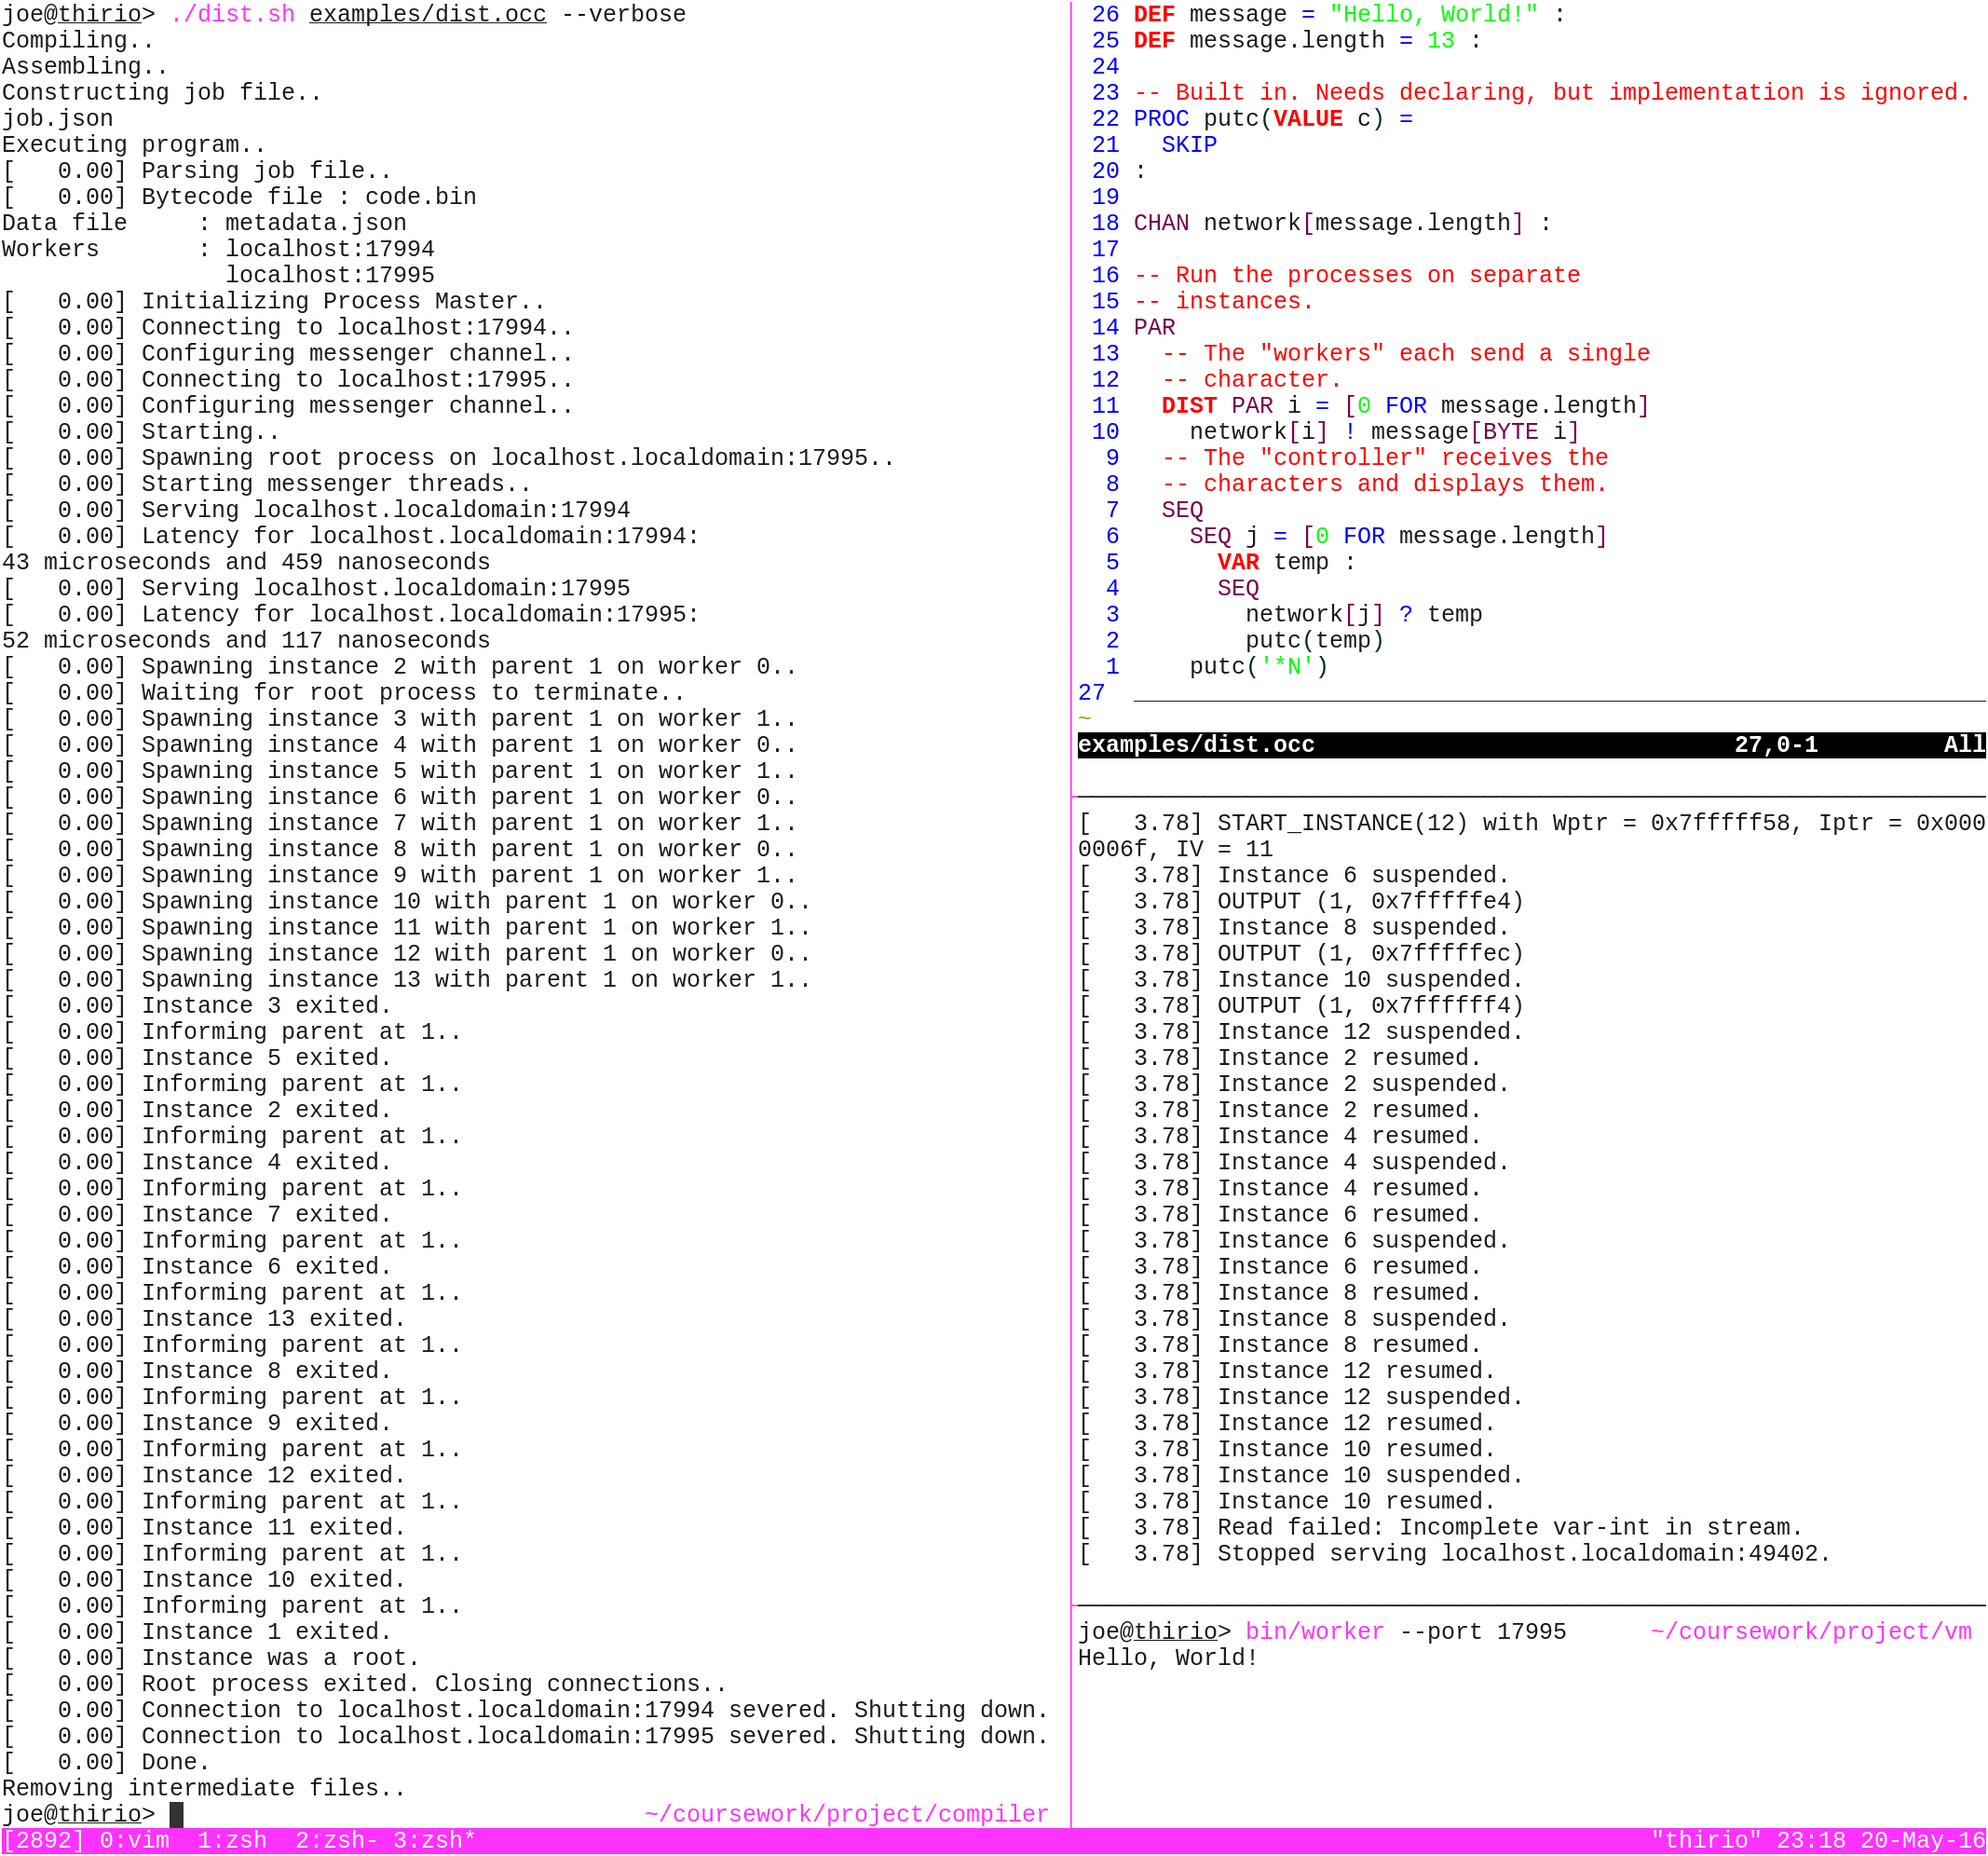
\includegraphics[width=\textwidth]{images/distributed}
      \caption{
        Running a distributed "Hello, World!" program on the distributed
        virtual machine with two workers. Left is master, top right is the program,
        middle right is the first worker (with --verbose), and bottom right is the
        second worker.
      }
    \end{figure}
    \begin{figure}[H]
      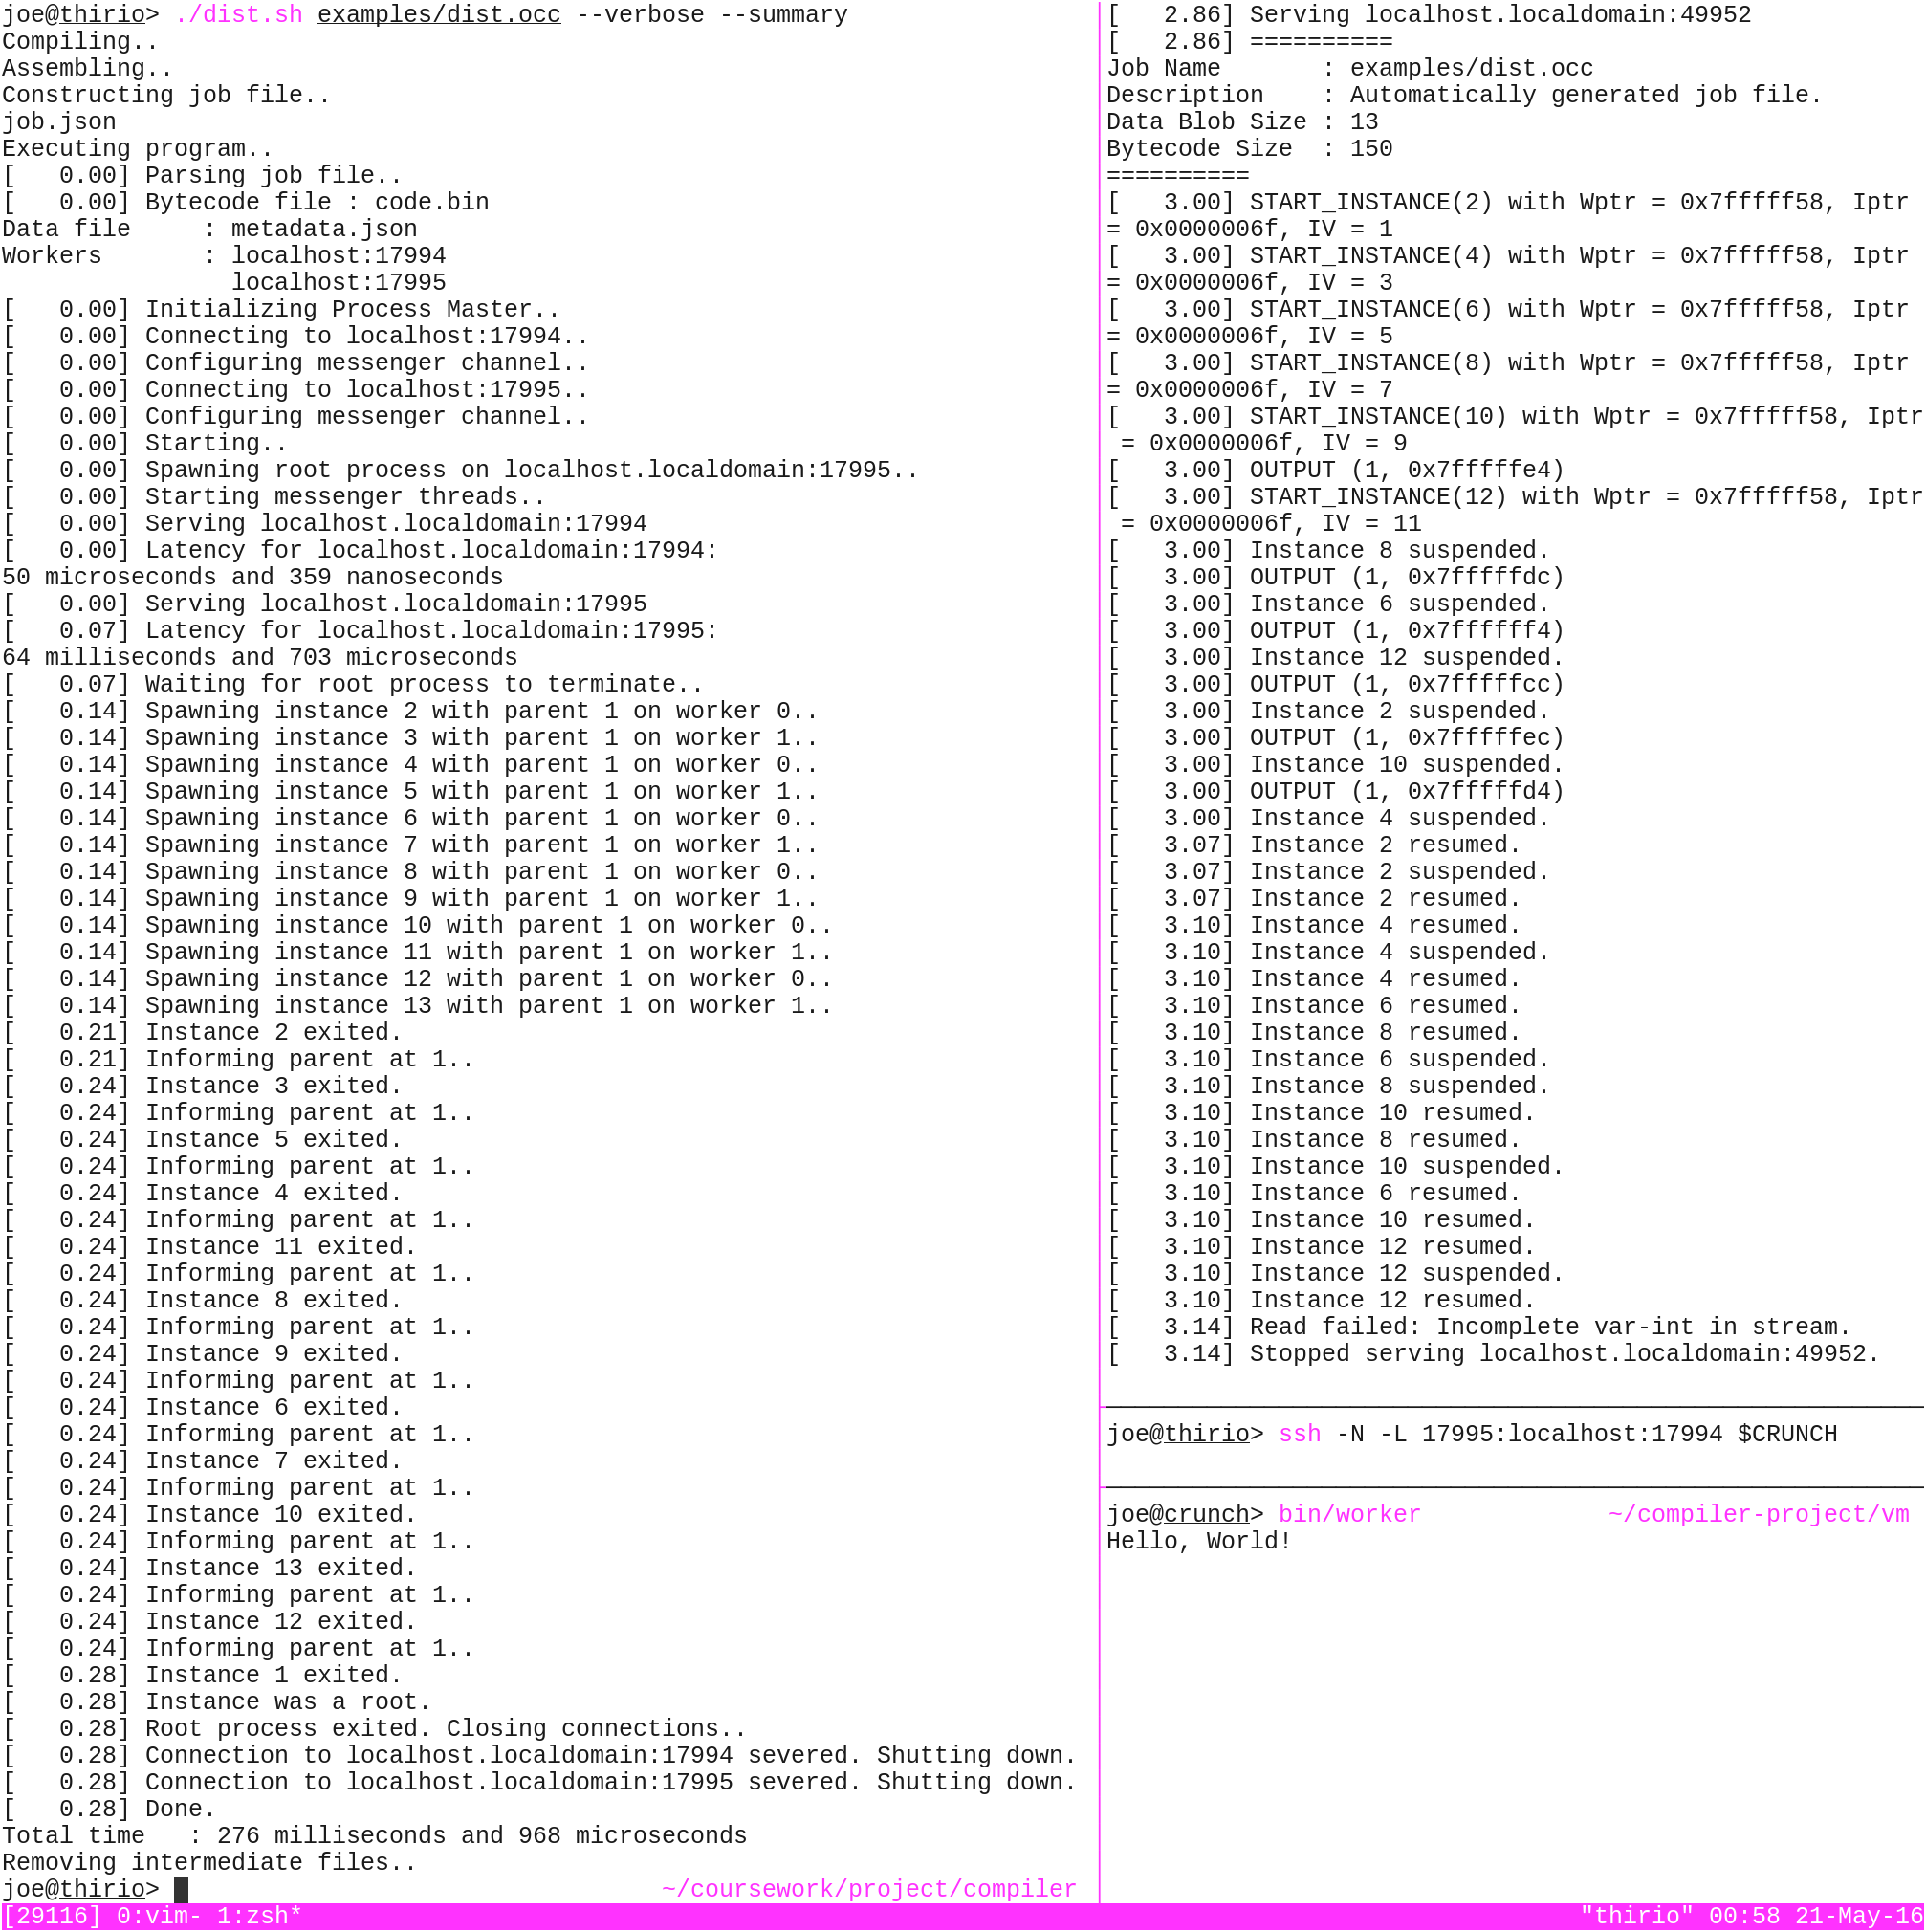
\includegraphics[width=\textwidth]{images/distributed_pi}
      \caption{
        Running the same distributed "Hello, World!" program, but with one of
        the workers running on a Raspberry Pi 3 which is 40 miles away.
      }
    \end{figure}
  
  \chapter{Replication in Occam} \label{adx-occam}
    In Occam, any of the \texttt{IF}, \texttt{SEQ}, or \texttt{PAR} constructs can
be \textit{replicated}. What this means depends upon the construct:
\lstinputlisting[language=occam]{code/if.occ}
Here, the \texttt{IF} statement on lines 5-7 is equivalent to the following:
\lstinputlisting[language=occam]{code/if2.occ}
As you can see, allowing replication on \texttt{IF} statements drastically
reduces the amount of code required in such cases, without complicating the
simple cases.

Applying replication to \texttt{SEQ} is roughly equivalent to a \texttt{for}
loop in C, while applying replication to \texttt{PAR} is like a \texttt{for}
loop which runs all of its iterations in parallel.


  \addcontentsline{toc}{chapter}{Glossary}
    \printglossaries

  \addcontentsline{toc}{chapter}{Bibliography}
    \bibliographystyle{plain}

\begin{thebibliography}{99}

\bibitem{jones}
  Geraint Jones.
  \textit{Programming in Occam}.
  Web Edition, 2001.

\bibitem{occ21}
  \textit{Occam 2.1 Reference Manual}.
  SGS-THOMSON Microelectronics Limited, 1995.

\end{thebibliography}

\end{document}
